% !TeX program = lualatex
\documentclass[]{article}

\usepackage{caption,subcaption,graphicx,float,url,amsmath,amssymb,amsthm,tocloft,cancel,thmtools,gensymb,braket,tikz-feynman}
\usepackage[toc,nonumberlist]{glossaries}
\usepackage{glossaries-extra}
\newcommand\numberthis{\addtocounter{equation}{1}\tag{\theequation}}

\newtheorem{thm}{Theorem}
\newtheorem{defn}[thm]{Definition}
\newtheorem{cor}[thm]{Corollary}
\newtheorem{lemma}[thm]{Lemma}
\graphicspath{{figs/}}
\widowpenalty10000
\clubpenalty10000
\setcounter{tocdepth}{2}
\tikzfeynmanset{compat=1.0.0}
%opening
\title{Theoretical Minimum\\Advanced Quantum Mechanics}
\author{Simon Crase}

\begin{document}

\maketitle

\begin{abstract}
These are my notes from the Advanced Quantum Mechanics lectures\cite{susskind2013advanced}  from Leonard Susskind's Theoretical Minimum series\cite{susskind2007theoretical}. Feynman diagrams were prepared using \emph{TikZ-Feynman} \cite{ellis2016tikz}.
\end{abstract}

\tableofcontents
\listoffigures
\listoftables
\listoftheorems


\section{Review and Introduction to Symmetry}

\subsection{Review of Quantum Mechanics}

\begin{itemize}
	\item States: $\ket{\psi}$ and $\bra{\psi}$
	\item Observables: $A=A^{\dag}$. An observable is represented by a Hermitian matrix.
	\item Eigenvalues represent values that can be measured: $A\ket{\alpha} = \alpha\ket{\alpha}$
	\item Inner product $\braket{\phi|\psi}$	
	\item Orthogonal $\braket{\phi|\psi}=0$
	\item Independent values $\braket{x|x^{\prime}}=0$
	\item Wave function $\braket{x|\psi} = \psi(x)$
	\item Probability $P(x)=\psi^*(x)\psi(x)$
	\item Momentum $p\psi(x)=- i \hslash \frac{\partial \Psi}{\partial x}$
	\item Evolution operator is Unitary $U(t)$: $\ket{\psi(0)} = \ket{\psi(t)}$
	\item $\braket{\phi|\psi}=\braket{\phi|U^{\dagger}U|\psi}$ i.e. $U^{\dagger}U=I$
	\item $U(\epsilon)= I + \epsilon G$, so $G=-G^{\dagger}$, $G=- i H$
	\item For general $t$, $U(t)=e^{- i H t}$
\end{itemize}

\begin{align*}
\psi(t+\epsilon) =& e^{-i \hslash \epsilon} \ket{\psi(t)}\\
=& (1- i \hslash \epsilon)\ket{\psi(t)}\\
\frac{\ket{\psi(t+\epsilon)} -\ket{\psi(t)} }{\epsilon}&= -i \hslash \ket{\psi(t)}\\
\frac{\partial \ket{\psi}}{\partial t} =& -i H \ket{\psi(t)} \text{, Time dependent Schr\"odinger Equation}\\
H \ket{\psi} =& E \ket{\psi}\text{, Time independent Schr\"odinger Equation}
\end{align*} 


\subsection{Introduction to Symmetry}

\begin{defn}[Symmetry]
	A symmetry is a transformation that doesn't change equations. 
\end{defn}
Rotational symmetry is one of the most important symmetries, as is translational symmetry.

\begin{thm}[A symmetry is a unitary operator that commutes with Hamiltonian]
	\begin{align*}
	V \ket{\psi} =& \ket{\psi^{\prime}} \text{is a symmetry}\numberthis \label{eq:symmetry}\\
	\iff&\\
	V H =& H V\numberthis \label{eq:symmetry:commute}
	\end{align*}
\end{thm}

\begin{proof}
	Suppose $\psi_1$ evolves to $\psi_2$:
	\begin{align*}
	\ket{\psi_1} \xrightarrow{U}& \ket{\psi_2} \text {or, equivalently}\\
	\psi_2 =& U \psi_1 \text{. Now, if $V$ really is a symmetry:} \numberthis \label{eq:psi_1}\\
	\ket{\psi_1^{\prime}} \xrightarrow{U}& \ket{\psi_2^{\prime}} \text {,  or}\\
	\psi_2^{\prime} =& U \psi_1^{\prime} \text{, so from (\ref{eq:symmetry}):}\\
	V\ket{\psi_2} =& U V \ket{\psi_1} \text{, or, using (\ref{eq:psi_1})}\\
	V U\ket {\psi_1} =& U V \ket{\psi_1} \text{. But $\ket{\psi_1}$ is an arbitrary state, so} \\
	V U =& U V \text{ i.e. so for small time $\epsilon$}\\
	V (I - i \epsilon H) =& (I - i \epsilon H) V \text{, whence}\\
	V H =& H V \text{, which is (\ref{eq:symmetry:commute})}
	\end{align*}
	Moreover the symmetry $V$ should transform mutually exclusive states into mutually exclusive states, whence it should preserve orthogonality, hence $V$ should be unitary. 
\end{proof}



Symmetries can be discrete or continuous.

\begin{itemize}
	\item Discrete
	\begin{itemize}
		\item Reflection
		\item interchange particles
	\end{itemize}
	\item Continuous
	\begin{itemize}
		\item rotation
		\item translation
	\end{itemize}
\end{itemize}

All continuous symmetries can be generated by $I-i \epsilon G$, for some Hermitean $G$ such that $[H,G]=0$.

E.g.
\begin{align*}
V \psi(x) = & \psi(x-\epsilon)\text{, shift right}\\
=& \psi(x) - \epsilon \frac{\partial \psi}{\partial x}\\
V =& I -  \epsilon \frac{\partial }{\partial x}\\
=& I - \frac{i \epsilon}{\hslash}P\\
G =& \frac{P_x}{\hslash}\text{, Generator of $x$ translation}
\end{align*}


\section{Symmetry groups and degeneracy}\label{seq:symmetry:degeneracy}

\subsection{Symmetry groups and degeneracy}

Symmetries are operations that you can do on a system which don't change:
\begin{itemize}
	\item the description;
	\item the phenomena;
	\item then energy levels, and value of the energy.
\end{itemize}

Examples of symmetry:
\begin{itemize}
	\item translation--doesn't change energy levels, Hamiltonian, or the Scro\"edinger equation;
	\item rotation;
	\item interchanging identical particles;
	\item crystal symmetry: translate one lattice spacing (not exact if crystal not infinite).
\end{itemize}
Some symmetries are more abstract than others; the more obvious symmetries come from the properties of space; homogeneity and isotropy.

\begin{defn}[Degeneracy of energy levels]
	If there is more than one state with given energy level, that energy level is called degenerate. We will see that it only happens when there is a symmetry: symmetries sometimes imply degeneracy, but not always.
\end{defn}

Degeneracy isn't a coincidence: symmetry sometimes implies degeneracy.

One application of symmetry is to analyze the energy of a system and see if it has energy levels that exactly match.


We will start with Rotation symmetry and think about a very simple system, a particle moving in a circle. If it can't leave the circle we can describe its position using an angle $\theta$. It has a wave function $\psi(\theta)$, such that $\psi^*(\theta)\psi(\theta)$ gives the probability of finding the particle at a particular point.

For a small counter-clockwise rotation:
\begin{align*}
\psi(\theta) \rightarrow & \psi(\theta - \epsilon)\\
\delta\psi =& - \epsilon \frac{\partial \psi}{\partial \theta} \text{, c.f. linear momentum}\\
=& -i \epsilon \big(-i \frac{\partial \psi}{\partial \theta}\big)
\end{align*}
Now defining the Angular Momentum operator $L$:
\begin{align}
- i \frac{\partial}{\partial \theta} \triangleq&\hslash L \text{, Hermitean--c.f. $P=-i\hslash \frac{\partial}{\partial x}$}\\
\delta\psi =& - \frac{i \epsilon}{\hslash} L \psi \text{, generator of rotation}
\end{align}
What are the Eigenvalues and Eigenvectors of Rotation?

\begin{align*}
L\ket{\psi} =& m \ket{\psi}\\
-i \hslash \frac{\partial \psi}{\partial \theta} =& m \psi\\
\psi(\theta) =& e^{\frac{i m \theta}{\hslash}}\text{. Now, we want $\psi$ single valued (symmetry!), i.e.}\\
\psi(\theta + 2\pi) =& \psi(\theta) \text{, so}\\
\frac{m}{\hslash}=&k\text{, some integer. But, by convention, redefine $m$}\\
L=& m \hslash \numberthis \label{eq:magnetic:quantum:number}
\end{align*}
This is the quantization of angular momentum.

\begin{defn}[Magnetic quantum number]
	The eigenvalue of $L$, $m$ in (\ref{eq:magnetic:quantum:number}) is known as the Magnetic quantum number.
\end{defn}

We expect that the energy will depend on the angular momentum. Now $m\ne 0 \implies E(m)=E(-m)$, so we have degeneracy. A magnetic field breaks this; rotational symmetry isn't enough for degeneracy, but adding reflection symmetry is sufficient (but need two non-commuting symmetries).

We will use $M$ to denote reflection symmetry. If we have reflection symmetry, $E(m)=E(-m)$, because the reflection of a system with specified angular momentum is a system with opposite angular momentum (Avoid calling reflection symmetry "mirror symmetry", as is this is used in string theory with a precise meaning).

The reflection of a magnetic field is not the same field, as it is an axial vector. Imagine a current generating a magnetic field going into the plane. If we reflect, the current goes in the opposite direction, as does the magnetic field.

\begin{thm}[Two symmetries that don't commute apply degeneracy]
	Suppose we have two symmetries, whose generators are $A$ and $B$.
	\begin{align*}
		[A,H]=&0 \text{, because it's a symmetry}\\
		[B,H]=& 0\\
		[A,B]\ne 0
	\end{align*}
	then...
\end{thm}
\begin{proof}
	\begin{align*}
		[A,B]=& i C  \text{. Need $i$ for $C$ to be Hermitean}
	\end{align*}
	\begin{lemma}[C commutes with H]
		$[C,H]=0$
	\end{lemma}
	\begin{proof}
		There are two cases: $C$ is a linear combination of $A$ and $B$, or $A$, $B$, and $C$ are independent. Since the lemma is trivial in the former case, we shall suppose the latter.
		\begin{align*}
		i[C,H] =& (AB)H - H(AB)\\
		=& AHB -HAB\\
		=& [A,H]B\\
		=&0
		\end{align*}
	\end{proof}
	
	TBP
\end{proof}

\begin{thm}[Reflection and rotation don't commute]
	If $M\psi(\theta) = \psi(-\theta)$, $ML \ne LM$
\end{thm}
\begin{proof}
	\begin{align*}
	MLe^{i m \theta} =& M m e^{i m \theta}\\
	=&m e^{- i m \theta}\\
	LMe^{i m \theta} =& L e^{- i m \theta}\\
	=& -m e^{- i m \theta}\\
	[M,L]e^{im\theta}=&2m e^{- i m \theta}
	\end{align*}
\end{proof}





\begin{defn}[Commutator algebra]
	Closure of $\{A,B,C,...\}$ under commutation.
\end{defn}

Collection of generators is an algebra.

\begin{defn}[abelian]
	A group of symmetries that all commute.
\end{defn}

\begin{defn}[non-abelian]
	A group of symmetries that isn't abelian.
\end{defn}

\subsection{An example: Angular Momentum}

Consider a classical orbit with energy $E$, Figure \ref{eq:aqm-2-1}. 	Is it degenerate? All we have to do is rotate it to see a new orbit with energy $E$: rotation about the y-axis has added a z-component. This is a classical suggestion that the quantum mechanical operators of angular momentum don't commute (rotation about 2nd axis converts rotation about 1st into something with a component along 3rd).

\begin{figure}[H]
	\begin{center}
		\caption{Degeneracy of Angular Momentum(classical)}\label{eq:aqm-2-1}
		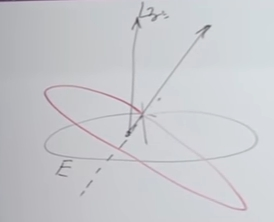
\includegraphics[width=0.5\textwidth]{aqm-2-1}
	\end{center}
\end{figure}

Let's look at the angular momentum generators. Figure \ref{fig:aqm-2-2} shows a  rotation about the z-axis by a small angle $\epsilon$.

\begin{figure}[H]
	\begin{center}
		\caption{Rotation in 2D by a small angle $\epsilon$}\label{fig:aqm-2-2}
		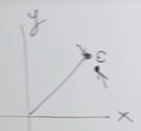
\includegraphics[width=0.5\textwidth]{aqm-2-2}
	\end{center}
\end{figure}

\begin{align*}
	\delta x =& - y \epsilon\\
	\delta y =& x \epsilon \text{. Now for a wave function $\psi(x,y)$}\\
	\delta \psi =& \frac{\partial \psi}{\partial x} \delta x + \frac{\partial \psi}{\partial y} \delta y\\
	=&\big( - y \frac{\partial \psi}{\partial x} + x \frac{\partial \psi}{\partial y}\big) \epsilon\\
	\triangleq& i \epsilon L_z \psi\\
	=& \big(- y P_x + x P_y x\big) i \epsilon \text{, whence}\\
	L_z =& x P_y - y P_x \text{, similarly}\\
	L_x =& y P_z - z P_y \text{, and}\\
	L_y =& x P_x - x P_z \text{, c.f. the classical formula}\\
	\vec{L} =& \vec{r} \times \vec{P}
\end{align*}
These are symmetries if the system is rotationally invariant.

Do they commute with each other? In \cite{susskind2014quantum} we saw
\begin{align*}
	[L,H_i]=& 0 \numberthis \label{eq:LH}\\
	[L_x,L_y] =& i L_z \numberthis \label{eq:lx_ly}\\
	[L_y,L_z] =& i L_x\numberthis \label{eq:ly_lz}\\
	[L_z,L_x] =& i L_y\numberthis \label{eq:lz_lx}
\end{align*}

\begin{defn}[Algebra]
	In mathematics, an \emph{algebra over a field } (often simply called an algebra) is a vector space equipped with a bilinear product. 
\end{defn}

\begin{defn}[Lie algebra]
	A Lie algebra is an algebra where multiplication is commutation. LS uses the definition that is is a collection of generators that is closed under commutation.
\end{defn}

So $L_x$, $L_y$, $L_z$ generate a Lie algebra: if we continue commuting we don't find anything new.

We want to find eigenvalues of angular momentum. It us useful to introduce creation and annihilation operators for $L_z$.
\begin{align*}
	L_{\pm} \triangleq& L_x \pm i L_y \numberthis \label{eq:comm:Lpm}\\
	[L_{\pm},L_Z] =& \mp L_{\pm} \numberthis \label{eq:comm:LpmLz}
\end{align*}

\begin{thm}[If $\ket{m}$ is an eigenvector of $L_z$, so are $L_+ \ket{m}$ and $L_- \ket{m}$]
	If 
	\begin{align*}
		L_z \ket{m} =& m \ket{m} \text{, then }\\
		L_z (L^+ \ket{m}) =& (m+1) (L^+\ket{m}) \text{, and}\\
		L_z (L^- \ket{m}) =& (m-1) (L^-\ket{m})
	\end{align*}
\end{thm}
\begin{proof}
	Suppose we have found one eigenvector of $L_z$:
	\begin{align*}
		L_z \ket{m} =& m \ket{m} \text{, magnetic quantum number}\numberthis \label{eq:ev:Lz}\\
		[L_+,L_z] \ket{m} =& \big(L_+L_z - L_zL_+\big) \ket{m}\\
		=&- L_+ \ket{m} \text{, from (\ref{eq:comm:LpmLz}). Rearranging  and using (\ref{eq:ev:Lz})}\\
		m L_+\ket{m} + L_+\ket{m} =& L_z L_+ \ket{m} \text{, whence}\\
		\big(m + 1 \big)L_+\ket{m}  =& L_z L_+ \ket{m} \text{; $L_+ \ket{m}$ is an eigenvector, eigenvalue $m+1$}\numberthis \label{eq:create_m}
	\end{align*}
	Similarly, $L_- \ket{m}$ is an eigenvector, eigenvalue $m-1$. The sequence of eigenvectors terminates if  $L_{\pm} \ket{m}=0$.
\end{proof}

So, using the algebra of commutators, we have generated a spectrum of values of $L_z$, separated by integers--see Figure \ref{fig:aqm-2-3}. Imagine that we rotate by $180\degree$: this takes $L_z\rightarrow - L_z$, so rotational symmetry requires that the termination points be reversed: they must be symmetrical. There are two possibilities--Figures \ref{fig:aqm-2-3a} and \ref{fig:aqm-2-3b}. We can show that the only values that are allowed for orbital angular momentum are integral (single values wave function), but half integral is also possible for spin. 

\begin{figure}[H]
	\caption{Spectrum of $L_z$.}
	\begin{subfigure}[t]{0.3\textwidth}
		\caption{Terminators in red}\label{fig:aqm-2-3}
		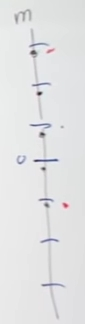
\includegraphics[width=0.8\textwidth]{aqm-2-3}
	\end{subfigure}
	\begin{subfigure}[t]{0.3\textwidth}
		\caption{Integral values in red}\label{fig:aqm-2-3a}
		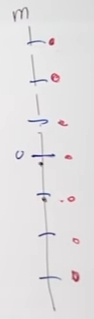
\includegraphics[width=0.8\textwidth]{aqm-2-3a}
	\end{subfigure}
	\begin{subfigure}[t]{0.3\textwidth}
		\caption{Half integral values}\label{fig:aqm-2-3b}
		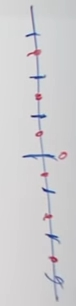
\includegraphics[width=0.8\textwidth]{aqm-2-3b}
	\end{subfigure}
\end{figure}

 We now show that the multiplet of states in Figure \ref{fig:aqm-2-3a} all have the same energy. 

\begin{thm}[Eigenvectors of $L_z$ are degenerate eigenvectors of $H$]
	\begin{align*}
	L_z \ket{m} = m \ket{m} \land& H \ket{m} = E \ket{m}\\
	 \implies&\\
	  H \ket{m \pm 1} =& E \ket{m \pm 1}
	\end{align*}
\end{thm} 
\begin{proof}
	\begin{align*}
	H \ket{m} =& E \ket{m} \numberthis \label{eq:assume_ev}\\
	H L_+ \ket{m} =& L_+ H \ket{m}\\
	=& L_+ E \ket{m} \text{, from (\ref{eq:assume_ev})}\\
	=& E L_+  \ket{m}\\
	H \ket{m+1} =& E \ket{m+1} \text{, from (\ref{eq:create_m})}
	\end{align*}
	Since symmetries commute, we have degeneracy.
\end{proof}

\section{Atomic orbits and harmonic oscillators}

\subsection{Atomic orbits and Angular Momentum}

We will talk more about what angular momentum is about.

If a particle moves in a central force field, angular momentum and, hence, the orbital plane are preserved. The state is $\psi(r,\theta,\phi)= \psi(r,\theta)$; if system were 2 dimensional, the angular momentum would be:

\begin{align*}
L =& -i \frac{\partial}{\partial \theta} \text{, and the eigenvalues and eigenvectors would satisfy}\\
-i \frac{\partial \psi(r,\theta)}{\partial \theta} =& l \psi(r,\theta) \text{, which has solution}\\
\psi(r,\theta) =& e^{i l \theta} \chi(r) \text{, for some $\chi$}
\end{align*}

In 3 dimensions, $\psi(r,\theta,\phi)= Y(\theta,\phi) \chi(r)$, where $Y(\theta,\phi)$ encapsulates the angular dependence of the wave function.

In Section \ref{seq:symmetry:degeneracy} we derived the commutators, (\ref{eq:lx_ly}), (\ref{eq:ly_lz}), and (\ref{eq:lz_lx}). We selected one component, $L_z$, and worked with its eigenvectors, $L_z \ket{m} = m \ket{m}$. We defined $L_\pm$, (\ref{eq:comm:Lpm}), and found that they had useful properties, (\ref{eq:comm:LpmLz}). $L_\pm$ were raising and lowering operators, which take use up and down the spectrum.

We asked whether the raising and lowering could go on forever. The only way to come to an end is if $\exists l$ such that $L_+\ket{k}=0$ (and similarly for $L_-$). Spectrum has to be symmetric (rotational invariance). We found spectrum had to go up in integers, and that it started at either an integer or half integer. We found that the spectrum was a multiplet of $2l+1$ states. The multiplet is characterized by the magnitude of angular momentum.


From (\ref{eq:create_m}) we have a spectrum of angular momenta, integral or half integral, say $\set{-l,...,l:L_+\ket{l}=0}$. There are $2l+1$ states with constant $L^2 = L_x^2 + L_y^2 + L_x^2$. Classically $L^2 = L_z^2 +(L_x-iL_y)(L_x+iL_y)$, but this fails in quantum mechanics as they operators don't commute.

The quantum version is:
\begin{align*}
	L^2 =& L_z^2 +(L_x-iL_y)(L_x+iL_y) -i [L_x,L_y]\\
	=& L_z^2 + L_z + L^-L^+\\
	L^2\ket{l}=& L_z^2\ket{l} + L_z\ket{l} + L^-L^+\ket{l}\\
	=& l^2\ket{l} + l\ket{l} + 0\text{, because eigenvectors.}\\
	L^2\ket{l}=&l (l+1) \ket{l} \numberthis \label{eq:max:L}
\end{align*}

\begin{thm}[Degeneracy of $L^2$]\label{thm:degeneracy:L2}
	\begin{enumerate}
		\item $[L^2, L_i] =0$\label{thm:degeneracy:1}
		\item All eigenvectors of $L_z$ are eigenvectors of $L^2$, eigenvalue $l(l+1)$\label{thm:degeneracy:2}
	\end{enumerate}
\end{thm}
\begin{proof}
	Part \ref{thm:degeneracy:1}
	\begin{align*}
		[L^2, L_x] =& [L_x^2+L_y^2+L_2^2,L_x]\\
		=& \cancel{[L_x^2,L_x]} + [L_y^2,L_x] + [L_z^2,L_x] \numberthis \label{eq:L2}\\
		[L_y^2,L_x]=&L_yL_yL_x -L_y L_x L_y + L_y L_x L_y -L_xL_yL_y\\
		=&-L_y[L_x,L_y]-[L_x,L_y]L_y\\
		=&-iL_yL_z-iL_zL_y \text{, using (\ref{eq:lx_ly})} \numberthis \label{eq:ly2x}\\
		[L_z^2,L_x]=&L_zL_zL_x -L_z L_x L_z + L_z L_x L_z -L_xL_zL_z\\
		=&L_z[L_z,L_x]+[L_z,L_x]L_z\\
		=&iL_zL_y+iL_yL_z \text{, using (\ref{eq:lz_lx})} \numberthis \label{eq:lz2x}\\
		[L^2, L_x] =&0 \text{, on substituing (\ref{eq:ly2x}) and (\ref{eq:lz2x}) in (\ref{eq:L2})}
	\end{align*}
	Part \ref{thm:degeneracy:2}. We know from (\ref{eq:max:L}) that the eigenvector of $L_z$ with the maximum eigenvalue satisfies the  theorem. The theorem follows by induction once we have the following Lemma.
	\begin{lemma}[Induction step for Theorem \ref{thm:degeneracy:L2}]
		If $\ket{m}$ is an eigenvector of $L_z$, and it is also an eigenvector of $L^2$, with eigenvalue $l(l+1)$, and $L_-\ket{m}$ is not zero, then  $L_-\ket{m}$ is an eigenvector of $L^2$, with eigenvalue $l(l+1)$.
	\end{lemma}
	\begin{proof}
		\begin{align*}
		L^2\ket{m}=&l (l+1) \ket{m} \text{, by hypothesis. Now}\\
		[L_-,L^2] =& 0 \text{, from (\ref{eq:comm:Lpm}) and Part \ref{thm:degeneracy:1}, hence}\\
		L^2(L_- \ket{m})=&(L^2 L_-) \ket{m}\\
		=& (L_- L^2) \ket{m}\\
		=& L_- (L^2 \ket{m})\\
		=& L_- [l (l+1) \ket{m}]\\
		=& l (l+1) (L_- \ket{m})
		\end{align*}
	\end{proof}
	
\end{proof}

When we find a multiplet such as Figure \ref{fig:aqm-2-3}, we not only have eigenvectors of $L_z$, but also of $L^2$. For each $l $, there are $2l+1$ states with the same $L^2$, and the same Energy\footnote{Because $[L_i,H]=0$--(\ref{eq:LH})}. Classically they are just tilts--Figure \ref{eq:aqm-2-1}.

We have a collection of functions of the angles, characterized by $m$ and $l$, $Y_{ml}(\theta,\phi)$. They are known as ''spherical harmonics'', and they are the analogues on the unit sphere of $e^{\pm i l \theta}$

\subsection{The Central Force Problem}

We will use classical mechanics to guess a solution.


Classically:
\begin{align*}
	H =& \frac{\vec{P}^2}{2m} + V(r) \text{, conserved} \numberthis \label{eq:classical:Hamiltonian}\\
	\vec{L} =& \vec{r}\times \vec{P}  \text{, angular momentum is conserved, so use $xy$ plane}\\
	H =& \frac{P_r^2+P_{\theta}^2}{2m} +V(r) \text{, resolving as shown in Figure \ref{fig:aqm-3-1-momentum}} \numberthis \label{eq:resolve}\\
	=& \frac{P_r^2}{2m} + \frac{L^2}{2m r^2} + V(r) \text{, since $\left|L\right| = \left|r\right| \left|P\right|$}
\end{align*}

So we have an equation for a one dimensional problem. Figure \ref{fig:aqm-3-central} depicts the potential, and Figure \ref{fig:aqm-3-central-osc} shows a solution, oscillations about the $r$ that yields the minimum potential. 

\begin{figure}[H]
	\caption{Central Force as  a one dimensional problem}
	\begin{subfigure}[t]{0.3\textwidth}
		\caption{Resolving momentum into radial and angular components}\label{fig:aqm-3-1-momentum}
		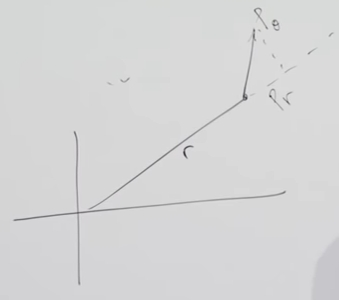
\includegraphics[width=\textwidth]{aqm-3-1-momentum}
	\end{subfigure}
	\begin{subfigure}[t]{0.3\textwidth}
		\caption{Potential assuming the Coulomb force}\label{fig:aqm-3-central}
		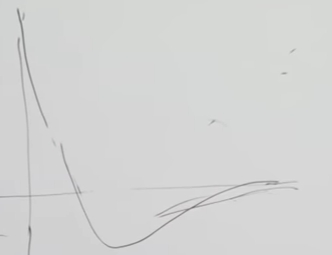
\includegraphics[width=\textwidth]{aqm-3-central}
	\end{subfigure}
	\begin{subfigure}[t]{0.3\textwidth}
		\caption{Small oscillations about minimum}\label{fig:aqm-3-central-osc}
		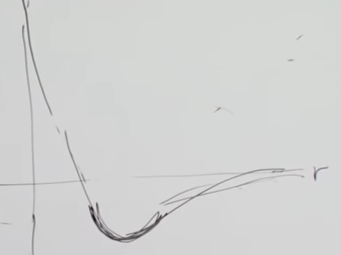
\includegraphics[width=\textwidth]{aqm-3-central-osc}
	\end{subfigure}
\end{figure}

That is the classical physics. What about the quantum physics? For the quantum physics we have a wave function which satisfies the Schr\"odinger Equation(\ref{eq:schroedinger:central}). The angular part is totally taken care of by our existing study of angular momentum\footnote{Strictly step (\ref{eq:resolve}) requires a quantum mechanical justification}.
\begin{align*}
	-\frac{\hslash^2}{2m}\frac{\partial^2 \psi(r)}{\partial r^2} + \hslash^2 \frac{l(l+1)\hslash^2}{r^2}\psi(r)+V(r)\psi(r) =& E\psi(r)\numberthis \label{eq:schroedinger:central}
\end{align*}

Figure \ref{fig:aqm-3-central-potential} depicts the potential for the Coulomb force. The energy levels of (\ref{eq:schroedinger:central}) are characterized by the number of nodes--Definition \ref{defn:node} and Figures \ref{fig:aqm-3-central-0node}, \ref{fig:aqm-3-central-1node}, and \ref{fig:aqm-3-central-2nodes} (The more nodes, the faster the wiggle, hence higher momentum).

\begin{figure}[H]
	\caption{Solving (\ref{eq:schroedinger:central})}
	\begin{subfigure}[t]{0.45\textwidth}
		\caption{Potential}\label{fig:aqm-3-central-potential}
		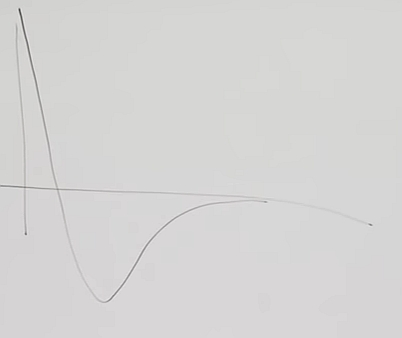
\includegraphics[width=\textwidth]{aqm-3-central-potential}
	\end{subfigure}
	\begin{subfigure}[t]{0.45\textwidth}
		\caption{No nodes}\label{fig:aqm-3-central-0node}
		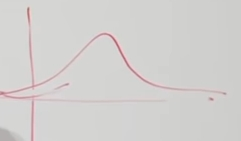
\includegraphics[width=\textwidth]{aqm-3-central-0node}
	\end{subfigure}
	\begin{subfigure}[t]{0.45\textwidth}
		\caption{One node}\label{fig:aqm-3-central-1node}
		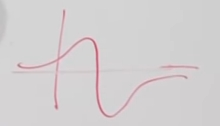
\includegraphics[width=\textwidth]{aqm-3-central-1node}
	\end{subfigure}
	\begin{subfigure}[t]{0.45\textwidth}
		\caption{Two nodes}\label{fig:aqm-3-central-2nodes}
		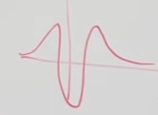
\includegraphics[width=\textwidth]{aqm-3-central-2node2}
	\end{subfigure}
\end{figure}

\begin{defn}[Node]\label{defn:node}
	A node is a point where the wave function is zero.
\end{defn}

\begin{thm}[Nodes and energy levels]
	The ground state has 0 nodes, the first excited one node, etc.
\end{thm}

What can we say about energy levels in general? Figure \ref{fig:degeneracy:hydrogen} plots the number of energy levels against $l$, and plots number of nodes vertically. It exhibits degeneracy. If the energy is too high the electron escapes. The Coulomb potential has a very special feature. It is almost an accident: it is violated by the finite size of the nucleus, by relativistic corrections, by spin. \emph{The zero node energy for $l=1$ is equal to the 1 node energy for $l=0$, etc}--Figure \ref{fig:aqm-3-central-coulomb}.



\begin{figure}[H]
	\begin{center}
		\caption[Degeneracy of Energy Levels in Hydrogen Atom]{Degeneracy of Energy Levels in Hydrogen Atom. Each $l$ has its own Schro\"edinger equation (\ref{eq:schroedinger:central}), so each $l$ may have its own set of bound solutions. The ground state for $l=0$ has no nodes,  the next state has one node, etc. For $l=1$ the energy of the ground state lies somewhere above the corresponding state for $l=1$. Moreover there are 3 states for each node: the energy levels are degenerate. Similarly for $l=2$ there are 5 states for each node, and the energy levels are higher.}\label{fig:degeneracy:hydrogen}
		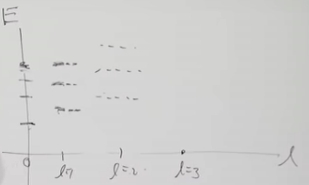
\includegraphics[width=0.9\textwidth]{aqm-3-hydrogen-degeneracy}
	\end{center}
\end{figure}

\begin{figure}[H]
	\begin{center}
		\caption[Energy Levels for the Coulomb Force]{For the Coulomb force \emph{only}, the energy levels for $l+1$ match those for $l$, shifted up by one. This is an extra degeneracy from a bizarre symmetry. The number of states at each level is  $\{1,4,9,16,...\}$}\label{fig:aqm-3-central-coulomb}
		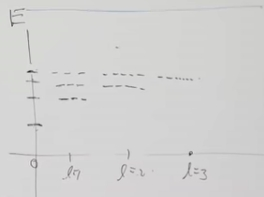
\includegraphics[width=0.8\textwidth]{aqm-3-central-coulomb}
	\end{center}
\end{figure}

Real atoms behave a bit differently.
\begin{itemize}
	\item the nucleus has finite size, so at short distances the Coulomb law isn't quite accurate;
	\item Instead of  $\{1,4,9,16,...\}$ states at each energy level there are  $\{2,8,18,32,...\}$--we have ignored \emph{spin}.
\end{itemize}



Are there always raising an lowering operators? No: only when you are very lucky; physics has been lucky twice. The harmonic oscillator piece of luck is very pervasive, as many things in nature can be well approximated by a harmonic oscillator. For example, go to a higher momentum state of the central force problem, Figure \ref{fig:aqm-3-central-osc}, and the simplest solution is to treat them as a harmonic oscillator.

\subsection{Harmonic oscillators}


Everything in physics that has an equilibrium, if you disturb equilibrium by a small amount, the behaviour can be approximated by a  harmonic oscillator. The model is just a suspended mass $(m=1)$, spring constant $(k=\omega^2)$

\begin{figure}[H]
	\begin{center}
		\caption[Model: suspended mass.]{Suspended mass $(m=1)$, spring constant $(k=\omega^2)$.  $X$ is deviation from equillibrium.}\label{fig:aqm-3-shm-suspended-mass}
		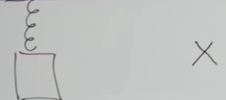
\includegraphics[width=0.8\textwidth]{aqm-3-shm-suspended-mass}
	\end{center}
\end{figure}

Classically:
\begin{align*}
	H =& \frac{P^2}{2m} + \frac{\omega^2 x^2}{2} \text{. We'll check with Hamilton's equations}\\
	 \dot{p}=&\frac{\partial H}{\partial x} \\
	=& \dot{x} \\
	\dot{x} =& -\frac{\partial H}{\partial p} \\
	=& - \omega^2 p \\
	\dddot{x} + \omega^2 x =&0 \text{, as expected}
\end{align*}

Quantum mechanically:
\begin{align*}
	H =& \frac{P^2}{2m} + \frac{\omega^2 x^2}{2}\\
	=& \frac{\omega}{2 \omega}\big(P + i \omega x \big)\big(P - i \omega x \big) - \frac{i \omega}{2} [x,P] \text{, since x and p don't commute}\\
	=& \frac{\omega}{2 \omega}\big(P + i \omega x \big)\big(P - i \omega x \big) + \underbrace{\frac{\hslash \omega}{2}}_\text{zero point energy}\\
	=&\omega \frac{\big(P + i \omega x \big)}{\sqrt{2 \omega}}\frac{\big(P - i \omega x \big)}{\sqrt{2 \omega}}
\end{align*}

Classically both $p=0$ and $x=0$ in the ground state; since the Heisenberg uncertainty principle precludes  $p=0$ and $x=0$, the zero point energy is the minimum possible. We'll drop the ground state energy (zero point energy) for the time being, since it is just an additive constant.

We'll introduce raising and lowering operators:

\begin{align*}
	a^+ \triangleq & \frac{P + i \omega x } {\sqrt{2 \omega}} \numberthis \label{eq:creation:operator}\\
	a^- \triangleq & \frac{P - i \omega x } {\sqrt{2 \omega}}\text{, Hermitean conjugate--$a^-=(a^+)^\dagger$} \numberthis \label{eq:annihilation:operator}\\
	H =& \omega a^+ a^-\text{. We'll take the commutator:}\numberthis \label{eq:shM}\\
	[a^-,a^+] =& \frac{1}{2\omega}\big[P - i \omega x,P + i \omega x\big]\\
	=& 1\text{. We also define} \numberthis \label{eq:a:comm}\\
	N \triangleq& a^+a^-\text{, so (\ref{eq:shM}) becomes} \numberthis \label{eq:number:operator}\\
	H =& \omega N
\end{align*}
$N$ is Hermitian, so it has a complete set of eigenvalues and eigenvectors.

\begin{align*}
	N\ket{n} =& n\ket{n} \text{, we aren't \emph{assuming} that $n$ is an integer}\\
	a^+a^-\ket{n} =& n\ket{n}\\
	a^+(a^-a^+ - a^+a^-)\ket{n} =& a^+\ket{n}\text{, using (\ref{eq:a:comm})}\\
	a^+a^-a^+ \ket{n} - a^+\underbrace{a^+a^- \ket{n}}_\text{$ n\ket{n}$} =& a^+\ket{n}\\
	\underbrace{a^+a^-}_\text{$N$}a^+ \ket{n} =& n a^+\ket{n} + a^+\ket{n}\\
	N a^+ \ket{n} =& (n+1) a^+ \ket{n}
\end{align*}

So $a^+$ acts as raising operator, and we can show $a^-$ is lowering.  Since the Hamiltonian is positive we can't ever get negative energy, so there must be a lowest energy state, $0$--Figure \ref{fig:aqm-3-spectrum}. In QM there is a theorem that all the eigenvalues of $MM^\dagger$ are positive or zero, for any operator $M$. 

\begin{figure}[H]
	\begin{center}
		\caption[Energy Spectrum for Harmonic Oscillator]{Energy Spectrum for Harmonic Oscillator. $a^+$ takes energy up one level, and $a^-$ down, except for $a^-\ket{0}$=0.}\label{fig:aqm-3-spectrum}
		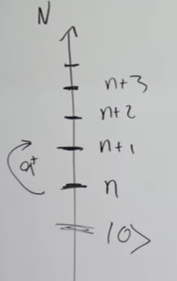
\includegraphics[width=0.8\textwidth]{aqm-3-spectrum}
	\end{center}
\end{figure}
We will see (Theorem \ref{thm:norm:harmonic}) the appropriate normalization gives:
\begin{align*}
	a^+\ket{n} =& \sqrt{n+1}\ket{n+1}\\
	a^-\ket{n} =& \sqrt{n}\ket{n-1}
\end{align*}
 
\section{Spin}

\subsection{Harmonic oscillators(continued)}

Harmonic oscillators are ubiquitous. Any time a system has an equilibrium, thee can be oscillations about equilibrium. An oscillator can oscillate at different frequencies simultaneously (harmonics)--e.g. a violin string. We will be particularly interested in oscillations in an electromagnetic field.  For example, if you have radiation in a cavity, there will be a variety of oscillations. What is the equilibrium? No electromagnetic field, i.e. vacuum is the equilibrium for electromagnetic field. Give it a knock, e.g. microwaves, and there will be oscillations.

In a crystal, the oscillations of one atom affect its neighbours, so we have a field. The quanta are called phonons.

In the previous lecture we found:
\begin{align*}
	H =& \frac{P^2}{2m} + \frac{\omega^2 x^2}{2} \text{, and we defined}\\
	a^\pm=& \frac{q \pm i \omega x}{\sqrt{2 \omega}} \text{, raising and lowering operators}\\
	[a^-,a^+]=& 1\\
	N =& a^+a^- \text{, whence}\\
	H =& \omega(N+\frac{1}{2})
\end{align*}

We will find ground state by solving the Schr\"odinger equation.
\begin{align*}
	\ket{psi} \rightarrow& \psi_0(x) \text{, in thr ground state}\\
	X \rightarrow& x. \text{, multiplication}\\
	P \rightarrow& -i \frac{d}{dx}
\end{align*}


We know that there has to be a ground state. We can't use $a^-$ indefinitely; since $H$ is positive, there can be no negative eigenvalues. So $\exists \ket{0}$ such that: 
\begin{align*}
	a^-\ket{0}=&0\\
	N\ket{0}=&a^+a^- \ket{0 }\\
	=& a^+0\\
	=&0
\end{align*}

NB $\ket{0} \ne 0$. $\ket{0}$ is a vector which can be normalized; $0$ is a vector of length 0.
Applying the transformations given above, we get the time independent Schr\"odinger equation.
\begin{align*}
	-\frac{1}{2}\frac{d^2 \psi(x)}{dx^2} + \omega^2 x^2 \psi(x)=& E\psi(x)
\end{align*}

 There are solutions for all $E$, but the solutions are not normalizable unless E is in the spectrum, Figure \ref{fig:aqm-3-spectrum}. So we impose the condition $\braket{\psi|\psi}=1$, or:
\begin{align*}
	\int_{-\infty}^{\infty} dx \psi^*(x) \psi(x) =& 1 \text{. We know that}\\
	a^-\ket{0}=& 0 \text{, whence}\\
	\big(-i \frac{d}{dx} - i \omega x \big)\psi_0(x) =& 0 \text{. Write}\\
	\psi(x)=&e^{f(x)} \text{, then}\\
	\psi^\prime(x) =&f^\prime e^{f(x)}\\
	i \big[f^\prime  + \omega x\big]e^{f(x)} =&0\\
	f(x) =& -\frac{\omega x^2}{2}+C\\
	\psi_0(x) =& e^{-\frac{\omega x^2}{2}} \text{, not normalized.}
\end{align*}

We can then use $a^+$  to generate excited states.
\begin{align*}
	\ket{1}=& a^+ \ket{0} \text{, or, in the Schro\"edinger representation:}\\
	\psi_1(x) =& \big(-i \frac{d}{dx} + i \omega x \big) e^{-\frac{\omega x^2}{2}}\\
	=& 2 i \omega e^{-\frac{\omega x^2}{2}}
\end{align*}

This is an odd function (antisymmetric)--Figure \ref{fig:wave:harmonic}. It has one node.

Figure \ref{fig:wave:harmonic} shows how higher levels have more wiggles (momentum) and are away from origin (more likely to be far away) most of time.

\begin{figure}[H]
	\caption{Wave functions for harmonic oscillator}\label{fig:wave:harmonic}
	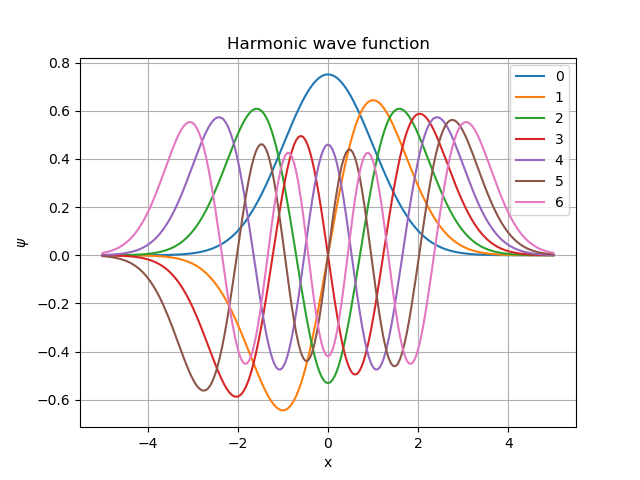
\includegraphics[width=0.9\textwidth]{harmonic_wavefunction}
\end{figure}

To see classical behaviour, superpose states to create wave packets. Time dependent looks like classical oscillator, especially at high energy (energy larger that ground state).

\url{https://youtu.be/ATxq2IEekk4?t=2504}

\subsection{Spin}

Some particles have half-integral spin, e.g. electron or proton. At rest has no orbital rotation, only spin. Spin is angular momentum attached to particle - see (\ref{eq:lx_ly}), (\ref{eq:ly_lz}), and (\ref{eq:lz_lx}). We introduce the Pauli matrices:

$$
\sigma_z = \begin{pmatrix}
1 & 0 \\
0 & -1
\end{pmatrix}
\quad
\sigma_x = \begin{pmatrix}
0 & 1 \\
1 & 0
\end{pmatrix}
\quad
\sigma_y = \begin{pmatrix}
0 & -i \\
i & 0
\end{pmatrix}
$$

then define:
\begin{align*}
s_i =& \frac{\sigma_i}{2} \text{. We can show the $s_i$ satisfy (\ref{eq:lx_ly}), (\ref{eq:ly_lz}), and (\ref{eq:lz_lx})}\\
[s_x,s_y] =& i s_z \\
[s_y,s_z] =& i s_x\\
[s_z,s_x] =& i s_y \text{. We define $J$, the total angular momentum}\\
J=&L+s
\end{align*}

Eigenvalues of $s_z$ are $\pm \frac{1}{2}$: notice that we have integral and half integral spins.


See Figure \ref{fig:degeneracy:hydrogen}. Number of states for each n, 1, 4, 9, 16, ...

For Helium, we can put 2 electrons into ground state; if we try to create an ion with 3 electrons, one goes into next state! Pauli exclusion principle. New property with two values, up and down. Checked with magnetic field.

Pauli's Exclusion Principle is a\emph{ postulate} of non-relativistic QM, but a \emph{consequence} of relativistic QM. There are two kinds of particles: ones that satisfy Pauli, and those that don't.

Identical quantum particles are indistinguishable.

\begin{align*}
\psi(x) =& \braket{x|\psi}\\
\psi(x_1,x_2) =& \braket{x_1x_2|\psi}\text{, two particles}\\
\psi(x_1,x_2) \rightarrow & \psi(x_2,x_1)\text{, swap using operator $S$}\\
S\ket{x1,x2} =& \ket{x2,x1}\\
S^2 =& 1
\end{align*}

$S$ is unitary, so eigenvalues are $\pm1$.

\section{Fermions: a tale of two minus signs}

Fermions: spin $\frac{1}{2}$ particles, which satisfy Pauli exclusion principle. NB, the 2 electrons in Helium are \textit{entangled}.

Photons don't have an exclusion principle; in fact they have a tendency to congregate.
 
Can we have spin $\frac{1}{2}$ particles that don't obey Pauli exclusion principle? No. Can show this from quantum field theory?

Consider wave function of positions for multiple particles, e.g. $\ket{x_1,x_2,x_3}$. Then $\braket{x_1,...x_n|\psi}=\psi(x_1,...x_n)$

\begin{align*}
\ket{x_1, x_2}=&\ket{x_2, x_1}e^{i\phi}\text{, interchange twice--there are two possibilities}\\
\ket{x_1, x_2}=&+\ket{x_2, x_1}\text{ Bosons}\\
\ket{x_1, x_2}=&-\ket{x_2, x_1}\text{ Fermions}
\end{align*}

NB: sign is not observable.

\begin{table}[H]
	\begin{center}
		\caption{Wave functions for Fermions and Bosons}
			\begin{tabular}{|l| l| l|} \hline 
				-&Fermions&Bosons \\ \hline 
				$\psi(x_1,x_2)=-\psi(x_2,x_1)$&Fermions&-\\ \hline
				$\psi(x_1,x_2)=\psi(x_2,x_1)$&-& Bosons\\ \hline
				$\psi_0(x_1)\psi_0(x_2)$&not OK& OK\\ \hline
				$\psi_0(x_1)\psi_1(x_2)$&not OK& not OK\\ \hline
				$\psi_0(x_1)\psi_1(x_2)+\psi_0(x_2)\psi_1(x_1)$&not OK& OK\\ \hline
				$\psi_0(x_1)\psi_1(x_2)-\psi_0(x_2)\psi_1(x_1)$&OK&not OK \\ \hline
			\hline
		\end{tabular}
	\end{center}
\end{table}


Rotate system by $2\pi$: is there a phase?

\begin{align*}
J_z\ket{\psi} =& -i \frac{\partial \ket{\psi}}{\partial \theta}\\
=& m\ket{\psi} \text{, if eigenvector}\\
\ket{\psi(\theta)} =& e^{im\theta}\ket{\psi(0)}\text{, so $m$ integral or half integral.}
\end{align*}

What if $m$ half integral and we rotate by $2\pi$? We have phase of $-1$, so $\psi$ changes sign.

David Finkelstein. Belt, Deep topological connection between rotation and interchange.

\section{Quantum Field Theory}

The description of nature as we know it, with the exception of gravity. In principle we believe that we could explain everything, except gravity, if we only had enough computational power.

\subsection{Review of Harmonic Oscillator}
Imagine many (possibly infinite number) harmonic oscillators.

From (\ref{eq:creation:operator}) and (\ref{eq:annihilation:operator}):
\begin{align*}
a^+_i \triangleq & \frac{P + i \omega x } {\sqrt{2 \omega}} \text{, creation operator} \numberthis \label{eq:creation:operator:i}\\
a^-_i \triangleq & \frac{P - i \omega x } {\sqrt{2 \omega}}\text{, annihilation operator} \numberthis \label{eq:annihilation:operator_i}\\
\end{align*}

Think of each oscillator  as an independent system of degrees of freedom, so operators commute. Using  (\ref{eq:a:comm}), and (\ref{eq:number:operator})

\begin{align*}
[a^+_i,a^+_j] =& 0 \numberthis \label{eq:a:comm_i_plus}\\
[a^-_i,a^-_j] =& 0 \numberthis \label{eq:a:comm_i_minus}\\
[a^-_i,a^+_i] =& \delta_{i,j} \numberthis \label{eq:a:comm_i}\\
H =& \hslash \sum_{i}  \omega_i N_i\text{, where $N_i$ are known as occupation numbers.}
\end{align*}
We're ignoring ground state energy.

One basis of states is $\ket{n_1,n_2,n_3,...}$.

\begin{thm}[Normalization of harmonic oscillator state--creation]\label{thm:norm:harmonic}
	\begin{align*}
	\left|\ket{n}\right|=&1\\
	\implies&\\
	a^+\ket{n}=&\sqrt{n+1}\ket{n+1}
	\end{align*}
\end{thm} 

\begin{proof}
	\begin{align*}
	a^+\ket{n}=&c_n\ket{n+1} \text{, fot the eigenvalue $c_n$}\\
	\bra{n}a^-=&c_n\bra{n+1}\text{, assume real}\\
	\braket{n|a^-a^+|n}=&c_n^2\text{, normalization!}\\
	=& \braket{n|a^+a^-+1|n}\text{, using (\ref{eq:a:comm_i})}\\
	=& \braket{n|N+1|n} \text{, from (\ref{eq:number:operator})}\\
	=&n+1 \text{, whence}\\
	c_n=&\sqrt{n+1}
	\end{align*}
\end{proof}

\begin{cor}[Normalization of harmonic oscillator state--annihilation]
	\begin{align*}
	a^-\ket{n}=\sqrt{n}\ket{n-1}
	\end{align*}
\end{cor}


$a_i^+\ket{n_1,n_2,.....}=\sqrt{n_i+1}\ket{n_1,n_2,...n_i+1,...}$

\subsection{Quantum Field Theory of Bosons}

Fields are functions of position. $\psi(x)$ not Hermitian, hence not an observable; we observe position, momentum, etc, but not $\psi$. $\psi(x_1,x_2,...x_{15})$ function of many positions. We want a quantity $\Psi$ such that:

\begin{itemize}
	\item $\Psi$ is an observable, e.g. magnetic field, so an operator.
	\item $\Psi$ function of one position
	\item $\Psi$ describes any number of particles.
\end{itemize}


Consider one particle in a box, and think about energy eigenstates. Wave function $\psi_1(x)$ is sine (lowest energy level). Next $\psi_2(x)$ has one node, with higher energy, $\psi_3(x)$ two nodes,...

Now many particles (bosons), some in first energy level, some in second,...$\ket{n1,n2,n3,...}$;  we invent operators as in (\ref{eq:a:comm_i_plus}) - (\ref{eq:a:comm_i}) to create and remove particles. NB $\set{1,2,3,...}$ are states $\set{n_i}$ occupation numbers.

\begin{align*}
(a^+a^-)\ket{n}=&(a^-a^+-1)\ket{n}\\
=&\sqrt(n+1)a^-\ket{n+1}-\ket{n}\\
=&(n+1)\ket{n}-\ket{n}\\
=&n\ket{n}
\end{align*}

NB: we are \text{ defining} creation and annihilation operators. Don't ask \emph{why} for a definition, \emph{ask why it is useful}. E.g. creation lets us create a photon. We want to study system with variable number of photons.

\begin{defn}[Vacuum]
	Vacuum is state that is annihilated by $a^-$ -- $\ket{0,0,0,....}$.
\end{defn}

Denote energy by $\omega_i$ for state $i$. 

\begin{align*}
E =& \sum_{i} n_i \omega_i\\
=& \sum_{i} \omega_i a^+_i a^-_i 
\end{align*}

We'll consider free particles--no interactions.

Why can we ignore ground-state energy? Because constants commute with everything. 

Quantum field theory is a book-keeping device for particles.

$\Psi(x)$ -- an operator that is a function of position--\emph{Fock Space}.

\begin{align*}
\Psi(x)\triangleq&\sum_{i}a^-_i\psi_i(x)\text{, not Hermitean, so conjugate is}\\
\Psi^\dagger(x)=&\sum_{i}a^+_i\psi_i^*(x)\\
\Psi(x)+\Psi^\dagger \text{ is}&\text{ Hermitean}
\end{align*}

What if we apply to vacuum? $\Psi(x)$ annihilates it--what about $\Psi(x)^\dagger$.

\begin{align*}
\sum_{i} \ket{i} \bra{i} =& I \text{, sum over states with $\psi_i$}\\
\sum_{i} \ket{i} \braket{i|X} =& \ket{X}\\
\psi^*_i(x)\underbrace{\ket{i}}_\text{one particle with state $i$} =& \ket{X}\text{, but}\\
\ket{i} =& a^+_i\ket{0} \text{, whence}\\
\psi^*_i(x) a^+_i\ket{0}=&\ket{x}\\
\Psi^\dagger(x) \ket{0} =& \ket{x}\text{ so $\Psi^\dagger(x)$ creates a particle at $x$.}
\end{align*}

\begin{itemize}
	\item $a^+_i$ creates a particle in state $i$.
	\item $\Psi^\dagger(x)$  creates a particle at position $x$.
	\item $a^-_i$ annihilates a particle in state $i$, or gives zero.
	\item $\Psi(x)$  annihilates a particle at position $x$, or gives zero.
\end{itemize}

There is a separate field for each Boson.

Add vacuum to a state, we get probability of 0.5 of vacuum, 0.5 of original state. It is not the same as zero. Vacuum has length of 1!

Let's add two particles, at $x$ and $y$. 
 
\begin{align*}
\Psi(y)\Psi(x)\ket{0} =& \ket{y,x}\\
\Psi(x)\Psi(y)\ket{0} =& \ket{x,y} \text{, but from (\ref {eq:a:comm_i_plus})}\\
\Psi(y)\Psi(x) =& \Psi(x)\Psi(y) \text{, so}\\
\ket{x,y} =& \ket{y,x} \text{, which is what we expect for Bosons.} 
\end{align*}

We can handle situation where number of particles is a random variable: a laser wave is a superposition.

\section{Quantum Field Theory II}

Can start with particles and see why they can be described by fields, or start with fields and quantize. Starting with particles we can use fields to handle variable numbers of particles. Normalization $\int \psi^*(x) \psi(x) dx=1$ gives \textit{number of particles}.

Given an orthonormal basis:
\begin{align*}
\sum_{i} \ket{i} \bra{i} =& I \text{, "Resolution of the Identity"}\numberthis \label{eq:resolution:identity}\\
\braket{y|x}=& \sum_{i} \braket{y|i} \braket{i|x}\\
\delta(x-y)=& \sum_{i} \psi_i(y) \psi^*_i(x)\text{, for any set of eigenvectors of Hermitan operator.}
\end{align*}

Can characterize multi-particle system by $\ket{n_1, n_2,...n_i,...}$. We want to increase and decrease occupation numbers, so introduce creation and annihilation operators.

\begin{itemize}
	\item $a^+_i=a^\dagger_i$
	\item $a^-_i=a_i$
\end{itemize} 

Introduce field operator
\begin{align*}
\Psi(x) \triangleq & \sum_{i} a_i \psi_i(x) \text{, would be Fourier if sine/cosine waves}\\
\Psi^\dagger(x) =& \sum_{i} a^\dagger \psi^*_i(x)\\
\Psi(x) + \Psi^\dagger(x) \text{ is}& \text{ Hermitean (observable)}\\
\frac{\Psi(x) - \Psi^\dagger(x)}{i} \text{ is}& \text{ Hermitean (observable)}
\end{align*}

Vacuum: $\ket{0} = \ket{0,0,0,.....}$.

\begin{align*}
\ket{x}=&\sum_{i}\ket{i}\braket{i|x}\text{, from (\ref{eq:resolution:identity})}\\
=& \sum_i \psi^*_i(x)a^\dagger_i\ket{0}\\
=& \Psi^\dagger(x) \ket{0}\text{, creation operator at a point.}
\end{align*} 

Consider the following operator:
\begin{align*}
\int dx \Psi^\dagger(x) \Psi(x)=&\int dx \sum_{i,j}a^+_i\psi_i^*(x) a_j\psi_j(x)\\
=&\sum_{i,j} a^+_i a_j \int dx \psi_i^*(x) \psi_j(x)\\
=&\sum_{i,j} a^+_i a_j \delta_{i,j}\\
=&\sum_i a^+_i a_i\\
=&\sum_i N_i\text{, operator representing total number of particles.}
\end{align*}

To make energy finite, total number of particles must be finite. $\Psi^\dagger(x) \Psi(x)$ represents particle density.

We now calculate the total energy.

\begin{align*}
E =& \sum_{i} N_i \omega_i\\
=& \sum_{i} a^\dagger_i a_i \omega_i
\end{align*}

We determine $\omega_i$ from eigenvalues of Schr\"odinger equation (ignoring interactions):
\begin{align*}
H \psi_i =& \omega_i \psi_i\\
\big[\frac{p^2}{2m} + V(x)\big]\psi_i(x)=& \omega_i \psi_i(x)\\
\big[-\frac{\nabla^2}{2m} + V(x)\big]\psi_i(x)=& \omega_i \psi_i(x)
\end{align*}

Guess solution
\begin{align*}
E=&\int dx \underbrace{\Psi^\dagger(x) \big[-\frac{\nabla^2}{2m} + V(x)\big] \Psi(x)}_\text{energy density} \\
=& \int dx \sum_{i,j}a^+_i\psi_i^*(x)\big[-\frac{\nabla^2}{2m} + V(x)\big]\psi_j(x)a^-_j\\
=& \int dx \sum_{i,j} a^+_i a^-_j \psi_i^*(x) \omega_j \psi_j(x)\\
=&  \sum_{i,j} a^+_i a^-_j \delta_{i,j} \omega_j
\end{align*}

Behaves like classical theory if the number of particles is very large. E.g. expectations follow classical laws.

If we don't split too many hairs, density from electromagnetic field is density of photons.

\section {Second Quantization}

\subsection{Digression on neutrinos}

If neutrinos have mass, and they mix, do they have the same mass? No.

How to mix and conserve energy?

Neutrinos - mass is energy. Eigenstates of energy are linear superpositions of eigenstates of something else, the type of neutrino. Eigenstates of energy don't mix with each other. Here is an analogous situation. Imagine a particle trapped in the potential of Figure \ref{fig:particle_mixed_left}, and assume middle barrier very high, so particle is trapped on one side or t'other (ignore tunnelling). What is ground state? But there must be a second ground state, from symmetry--Figure \ref{fig:double:well}.

\begin{figure}[H]
	\caption{Double well potential}
	\begin{subfigure}{0.5\textwidth}
		\caption{Double well potential}\label{fig:particle_mixed_left}
		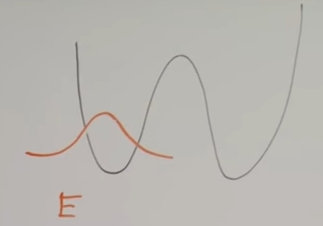
\includegraphics[width=0.8\textwidth]{particle_mixed_left}
	\end{subfigure}
	\begin{subfigure}{0.5\textwidth}
		\caption{Particle trapped in double well}\label{fig:double:well}
		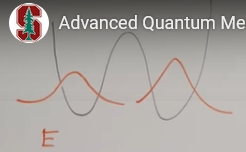
\includegraphics[width=0.8\textwidth]{particle_mixed}
	\end{subfigure}
\end{figure}



\begin{thm}[If $V$ is an even function, $\psi$ is either even or odd.]
	If  $\psi$  is a continuously differentiable solution to the time independent Schr\"odinger equation
	\begin{align*}
	-\frac{\hslash^2}{2m}\frac{d^2 \psi(x)}{d x^2} + V(x)\psi(x) =& E\psi(x) \text{ and}\numberthis \label{eq:ti:schroedinger}\\
	\forall x V(-x) =& V(x) \numberthis \label{eq:even_V}\\
	\text{then}&\text{ either}\\
	\psi(x) =& \psi(x)\text{, or}\\
	\psi(x) =& \psi(-x)
	\end{align*}
\end{thm}

\begin{proof}
	Define an operator $R$ (reflection in time) such that:
	\begin{align*}
		R \ket{\psi} =& \ket{\psi^{\prime}} \text{, where} \numberthis \label{eq:reflection}\\
		\psi^{\prime}(x) =& \psi(-x)
	\end{align*}
	
	(\ref{eq:even_V}) $\implies RV=V$, and $\psi^{\prime}$ satisfies (\ref{eq:ti:schroedinger}), whence:
	
	\begin{align*}
	\psi^{\prime}(x) =& \rho \psi(x) \text{, for some constant $\rho$.} \numberthis \label{eq:R:rho}
	\end{align*}
	WLOG we can assume that $\psi$ and $\psi^{\prime}$ are both normalized, whence:
	\begin{align*}
		\lvert \rho \rvert = 1& \text{, so (\ref{eq:reflection}) and (\ref{eq:R:rho}) give:}\\
		R \ket{\psi} =& \rho \ket{\psi} \text{. But (\ref{eq:reflection}) implies}\\
		R^2    =& I \text{, whence}\\
		\rho^2 =& 1 \text{, i.e.}\\
		\rho \pm& 1 \text{, so, in any interval where $\psi(x)\ne 0$ \emph{either}}\\
		\psi(x) =& \psi(-x) \text{\emph{or}}\\
		\psi(x) =& -\psi(-x)
	\end{align*}
	We still need to rule out the possibility that $\rho$ changes sign at a zero. Let $x_0$ be a point such that $\psi(x_0)=0$, and, WLOG, assume that $\psi(x)=\psi^{\prime}(x)$ in some interval up to $x_0-$ and $\psi(x)=-\psi^{\prime}(x)$ in some interval starting $x_0+$. Since $\psi$ is continuously differentiable: then $\frac{\psi^{\prime}(x_0-)}{dx}=\frac{\psi^(x_0-)}{dx}$. Now define $\psi^{\prime\prime} \triangleq \big(\psi^{\prime}-\psi\big)$: $\psi^{\prime\prime}$ satisfies (\ref{eq:ti:schroedinger}), $\psi^{\prime\prime}(x_0)=0$, and $\frac{\psi^{\prime\prime}(x_0-)}{dx}=0$, whence $\psi^{\prime\prime}=0 \forall x$. 
\end{proof}

But neither LHS or RHS wave function of Figure \ref{fig:double:well} symmetric or antisymmetric. Can make symmetric or antisymmetric combinations. Figure \ref{fig:double:well:symmetrized} has slightly lower energy than Figure \ref{fig:double:well}. Figure \ref{fig:double:well:1st} shows first excited state.

\begin{figure}[H]
	\caption{Wave functions for Figure \ref{fig:double:well}}
	\begin{subfigure}{0.45\textwidth}
			\caption{Wave function symmetrized(minimum in middle is slightly greater than zero-allow tunnelling)}\label{fig:double:well:symmetrized}
			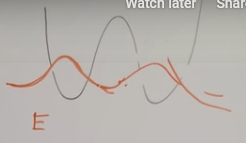
\includegraphics[width=0.8\textwidth]{particle_mixed_symmetrized}
	\end{subfigure}
	\begin{subfigure}{0.45\textwidth}
		\caption{First excited state}\label{fig:double:well:1st}
		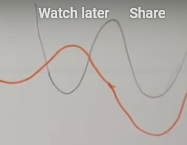
\includegraphics[width=0.8\textwidth]{particle_mixed_1st_excited}
	\end{subfigure}
\end{figure}


So we mix the pure states from Figures \ref{fig:double:well:symmetrized} and \ref{fig:double:well:1st}. Let's start with electron on left, and evolve.
\begin{align*}
\frac{\psi_L+\psi_R}{\sqrt{2}}& \text{--symmetric, with energy }& E_1-\epsilon\\
\frac{\psi_L-\psi_R}{\sqrt{2}}& \text{--antisymmetric, with energy }& E_1+\epsilon
\end{align*}
Each is an eigenvector, so they evolve as follows:
\begin{align*}
\frac{\psi_L+\psi_R}{\sqrt{2}} e^{(E_1-\epsilon)t}=&\psi^+ \text{, say}\\
\frac{\psi_L-\psi_R}{\sqrt{2}}e^{(E_1+\epsilon)t}=&\psi^-
\end{align*}

Now what if we start with pure $\psi_L$?
\begin{align*}
	\psi_L =& \frac{\psi^+ + \psi^-}{\sqrt{2}}\text{, then the denominator evolves as}\\
	\psi_L^\prime =&\psi^+ e^{(E_1-\epsilon)t} + \psi^- e^{(E_1+\epsilon)t}\\
	=&e^{E_1 t}\big[\psi^+ e^{-\epsilon t} + \psi^- e^{+\epsilon t}\big]
\end{align*}
Signs change with time, so eventually they will be opposite.
\begin{align*}
e^{-\epsilon t} =& - e^{\epsilon t}\\
e^{2 \epsilon t}=&-1\\
2 \epsilon t = \pi \text{, so $\psi_L$ becomes $\psi_R$!}
\end{align*}

Mixing goes with oscillation. Neutrinos go like that--electron neutrino changes to muon neutrino. Masses are energy levels. Coupling in Hamiltonian.

Ammonia is analogous: $N$ tunnels through $H_3$ plane. 

Spins.



\subsection{Second Quantization of Bosons}

Fourier transforms let us move between the position and momentum representations.

\begin{align*}
\psi(x) \rightarrow& \psi^*(x)\psi(x)=&P(x) \text{ in position representation}\\
\widetilde{\psi}(p) \rightarrow& \widetilde{\psi}^*(p) \widetilde{\psi}(p) =&P(p) \text{ in momentum representation, where}\\
\widetilde{\psi}(p) =& \int \frac{dx}{\sqrt{2\pi}} \psi(x) e^{-i p x}\\
\psi(x) =& \int \frac{dp}{\sqrt{2\pi}} \widetilde{\psi}(p) e^{+i p x}
\end{align*}

Now consider this in field theory.

\begin{align*}
\Psi(x) =& \sum_{i} a^-_i \psi_i(x)\\
\psi_i(x) =& e^{ipx} \text{ for a free particle (different $i$!), so} \\
\Psi(x)=& \int \frac{dp}{\underbrace{\sqrt{2\pi}}_\text{by convention}} a^-(p) e^{ipx} \text{, where annihilation operator}\\
a^-(p)& \text{ removes 1 particle with momentum p: plays same role as $\widetilde{\psi}(p)$ }\\
\Psi^\dagger(x)=& \int \frac{dp}{\sqrt{2\pi}} a^+(p) e^{ipx} \text{ creates particle at position $x$}
\end{align*}

There is a similarity between wave functions in position and momentum space and creation and annihilation operators for particles and given position or momentum.
\begin{align*}
a^-(p) = \int \frac{dx}{\sqrt{2\pi}} \Psi(x) e^{-ipx}\\
a^+(p) = \int \frac{dx}{\sqrt{2\pi}} \Psi^\dagger(x) e^{ipx}
\end{align*}

Remember there is a field operator for each kind of particle.

Can prove following.
 
\begin{align*}
[\Psi^+(x),\Psi^-(y)] =& \delta(x-y) \text{, introduces Heisenberg uncertainty!}\\
[\Psi^+(x),\Psi^+(y)] =&0\\
[\Psi^-(x),\Psi^-(y)] =&0\\
[\Psi^+_R(x),\Psi^-_I(y)] =& \delta(x-y) \text{, can not measure simultaneously at same point!}
\end{align*}

Makes sense in relativity: would violate causality. Spacelike! Can measure at different points.

Fermions don't work like this! One measurement can kick another arbitrarily far away.

\section{Quantum Field Hamiltonian}

\subsection{Particle Field Interactions}

Hamiltonian for very simple quantum field--particles satisfying Schr\"odinger equation. The second term counts particles, giving each energy $V(x)$.
\begin{align*}
H =& \int dx \big[ \Psi^\dagger(x) \big[\frac{- \nabla^2}{2m} \Psi(x) \big]+ V(x) \Psi^\dagger(x) \Psi(x) \big] \\
&\text{We restrict to the special case of constant potential energy}\\
H=&\int dx \big[\Psi^\dagger(x) \big(\frac{- \nabla^2}{2m} \Psi(x)\big) + mc^2 \Psi^\dagger(x) \Psi(x)\big]  \numberthis\label{eq:psi_mc2}
\end{align*}

The Hamiltonian updates state.

\begin{align*}
\ket{\phi(t+\epsilon)} =& (1-i \epsilon H) \ket{\phi(t)} \text{State}\\
=& \ket{\phi(t)} -i \epsilon H \ket{\phi(t)} \numberthis \label{eq:update:state}
\end{align*}

What would it mean to say momentum is conserved? It means Hamiltonian doesn't change momentum. Let's see how this works with (\ref{eq:psi_mc2}). Rewrite 2nd term  using momentum variables

\begin{align*}
\Psi(x) =& \int \frac{dp}{\sqrt{2\pi}} \widetilde{\Psi}(p) e^{ipx}\\
\Psi^\dagger (x) =& \int \frac{dp}{\sqrt{2\pi}} \widetilde{\Psi^\dagger}(p) e^{-ipx} \numberthis \label{eq:psi:dagger}\\
\int dx \big(mc^2\big) \Psi^\dagger(x) \Psi(x) =& \frac{mc^2}{2 \pi} \int \widetilde{\Psi^\dagger}(p_2) \widetilde{\Psi}(p_1) e^{i(p_1-p_2)x} dx dp_2 dp_1\\
=& \frac{mc^2}{2 \pi} \int \widetilde{\Psi^\dagger}(p_2) \widetilde{\Psi}(p_1) \delta(p_1-p_2) dp_2 dp_1\\
=& \frac{mc^2}{2 \pi} \int \widetilde{\Psi^\dagger}(p) \widetilde{\Psi}(p) dp
\end{align*}
This just removes a particle with momentum $p$ and puts it back; momentum isn't changed. Let's repeat with the 1st term of (\ref{eq:psi_mc2}.)

(Digression: calculation with multiple particles shows momentum still conserved.)

\begin{align*}
- \nabla^2 \Psi^\dagger (x) =& \int \frac{dq}{\sqrt{2\pi}} q^2 \widetilde{\Psi^\dagger}(q) e^{-iqx}\text{, from (\ref{eq:psi:dagger}), so}\\
\int dx \Psi^\dagger(x) \frac{- \nabla^2}{2m} \Psi(x)=& \int \frac{ p^2}{2m} \widetilde{\Psi^\dagger}(p) \widetilde{\Psi}(p) dp \text{, adds up kinetic energy.}
\end{align*}

Imagine two species of particles: fake electrons and protons that happen to be bosons.

\begin{align*}
H =& \int dx  \Psi^\dagger_e(x) \frac{- \nabla^2}{2m_e} \Psi_e(x) + \int dx \Psi^\dagger_p(x) \frac{- \nabla^2}{2m_p} \Psi_p(x)  + g \int dx \underbrace{\Psi^\dagger_e(x) \Psi^\dagger_e(x) \Psi_e(x) \Psi_p(x)}_\text{Figure \ref{fig:scatter:e:p}} \text{, where}\\
g=& \textit{ coupling constant--proportional to probability of interaction.}
\end{align*}

\feynmandiagram{};

\begin{figure}[H]
	\begin{center}
		\caption[$\Psi^\dagger_e(x) \Psi^\dagger_e(x) \Psi_e(x) \Psi_p(x)$--scattering]{$\Psi^\dagger_e(x) \Psi^\dagger_e(x) \Psi_e(x) \Psi_p(x)$: annihilate and create an electron and proton if they are at the same place, then create again --i.e. scatter}\label{fig:scatter:e:p}
		\feynmandiagram[vertical=o1 to i1]{
			i1[particle=$e^-$]--[fermion]a--[fermion]o1[particle=$e^-$],
			i2[particle=$e^+$]--[anti fermion]a--[anti fermion]o2[particle=$e^+$]
		};
	\end{center}
\end{figure}

\begin{itemize}
	\item Total momentum is conserved, not that of individual particles.
	\item Coulomb potential has been ignored.
	\item If experiment shows that particles interact, then there must be a term in the Hamiltonian.
\end{itemize}

Imagine particle decay, as shown in Figure \ref{fig:particle:decay}. We might try a term: $\Psi^\dagger_b(x) \Psi^\dagger_c(x) \Psi_a(x)$. Since space it isotropic, the interaction can happen anywhere: $g \int \Psi^\dagger_b(x) \Psi^\dagger_c(x) \Psi_a(x) dx$. We can show that momentum is conserved.

\begin{figure}[H]
	\begin{center}
		\caption{Particle Decay: $\Psi^\dagger_b(x) \Psi^\dagger_c(x) \Psi_a(x)$}\label{fig:particle:decay}
		\feynmandiagram[horizontal' = b to c]{
			a[particle=a]--[charged scalar]cc--[charged scalar]b[particle=b],
			cc--[charged scalar]c[particle=c]
		};
	\end{center}
\end{figure}

Now what goes in the Hamiltonian must be Hermitian, so we need:
\begin{align*}
g \int \Psi^\dagger_b(x) \Psi^\dagger_c(x) \Psi_a(x) dx + g \int \Psi^\dagger_a(x) \Psi_c(x) \Psi_a(x)
\end{align*}
which reverses the process of  Figure \ref{fig:particle:decay}: $b+c\rightarrow a$.
We now have a simple version of quantum field theory:
\begin{itemize}
	\item Creation and annihilation operators;
	\item Fields made out of creation and annihilation operators;
	\item Fields are functions of position;
	\item Each type of particle has its own field;
	\item Write down Hamiltonian with kinetic energies of particles and other concoctions. 
\end{itemize}

Imagine that we made $\epsilon$ a little larger in (\ref{eq:update:state}):

\begin{align*}
\ket{\phi(t+\epsilon)} =& \ket{\phi(t)} -i \epsilon H \ket{\phi(t)} - \frac{\epsilon^2}{2} H^2 \ket{\phi(t)}
\end{align*}

What is the effect of $H^2$? E.g., Figure \ref{fig:particle:decay} becomes a scatter: $b+c \rightarrow a \rightarrow b + c$. Or Figure \ref{fig:scatter:annihilate} shows a more complex situation. You can have a forest of interactions that are mediated by a single term in the Hamiltonian.

\begin{figure}[H]
	\begin{center}
		\caption{Exchange diagram}\label{fig:scatter:annihilate}
		\feynmandiagram[vertical=o1 to i1]{
			i1[particle=a]--[fermion]n1--[fermion]o1[particle=b],
			i2[particle=b]--[fermion]n2--[fermion]o2[particle=a],
			n1--[boson,edge label=c]n2
		};
	\end{center}
\end{figure}

Figure \ref{fig:scatter:annihilate} has a coupling constant $g^2$.


\begin{figure}[H]
	\caption[Scatter electron and emit photon(field $A$):$A\Psi^+_e\Psi^-_e$]{Scatter electron and emit photon(field $A$):$A\Psi^+_e\Psi^-_e$. Sometimes what you thought was an electron behaves like an electron + photon. Low probability: think of as correction to electron, not a new process. If we look, we will screw up electron! Superposition.}
	\begin{center}
		\begin{subfigure}{0.45\textwidth}
		\feynmandiagram[vertical=e2 to e1]{
			e1[particle=$e^-$]--[fermion]e2[particle=$e^-$]
			--[fermion]e3[particle=$e^-$],
			e2--[photon]x
		};
		\end{subfigure}
		\begin{subfigure}{0.45\textwidth}
			\feynmandiagram[vertical=e4 to e1]{
				e1[particle=$e^-$]--[fermion]e2--[fermion]e3
				--[fermion]e4[particle=$e^-$],
				e2--[photon,looseness=3.0,half left]e3
			};
		\end{subfigure}
	\end{center}
\end{figure}

\subsection{The Dirac Equation}

We will study the relativistic electron. We will start with an electron that moves in 1 direction along a line. Why did Dirac want to handle the relativistic case? Electrons in at atom move at a significant proportion of the speed of light.  

\begin{align*}
E =& \frac{p^2}{2m} \text {, classical}\\
P =& -i \frac{\partial}{\partial x} \text{, quantum}\\
H = & i \frac{\partial}{\partial t}\\
E^2 =& p^2 + m^2 \text{, relativistic($c^2=1$). This becomes:}\\
-\frac{\partial^2}{\partial t^2} \phi(x) =& -\frac{\partial^2}{\partial x^2}\phi(x) + m^2 \phi(x) \text{, Klein-Gordon equation. But Dirac wanted this:}\\
i \frac{\partial \psi}{\partial t} =& H\psi\\
=& \sqrt{- \frac{\partial^2}{\partial x^2} + m^2} \psi \text{. What could this mean?}  
\end{align*}

Dirac decided to start again. Imagine a particle moving along the x axis with the speed of light.

\begin{align*}
P =& E \text{, moving to right}\\
i \frac{\partial \psi}{\partial t} =& -i \frac{\partial \psi}{\partial x}\\
\implies&\\
\frac{\partial \psi}{\partial t} + \frac{\partial \psi}{\partial x}=&0\text{. Any function of x-t will satisfy equation}
\end{align*}

Three things are wrong with this equation:
\begin{enumerate}
	\item Allows particles with negative energy with negative momentum.
	\item Only has particles that move to the right.
	\item Electron has no mass: speed of light.
\end{enumerate}

Dirac solved second problem by imagining two species of electrons, one moving to the right, t'other to the left, labelled $\psi_1$ and $\psi_2$. Or a particle can be one or t-other, or a superposition.

\begin{align*}
\frac{\partial \psi_1}{\partial t} + \frac{\partial \psi_1}{\partial x}=&0\\
\frac{\partial \psi_2}{\partial t} - \frac{\partial \psi_2}{\partial x}=&0
\end{align*}

Imagine particle with two degrees of freedom, $x$ and $1/2$. Make second degree into matrix index. Introduce an observable, $\alpha$, to tell is whether particle is 1 or 2.

\begin{align*}
\underbrace{
	\begin{pmatrix}
		1 & 0\\
		0 & -1
	\end{pmatrix}
}_\text{Dirac's $\alpha$}
\begin{pmatrix}
	\psi_1\\
	\psi_2
\end{pmatrix}\\
H =& \alpha P\\
i\frac{\partial \psi}{\partial t} =& -i \alpha \frac{\partial \psi}{\partial x} \text{, matrix equation!}
\end{align*}

Dirac added a term to give electron mass. Then:

\begin{align*}
H =& \alpha P + \beta m \text{, where $\beta$ is some matrix. Now}\\
E^2 =& P^2 + m^2 \text{, so}\\
E^2 =& \big(\alpha P + \beta m \big) \big(\alpha P + \beta m \big)\\
=& \underbrace{\alpha^2 P^2}_\text{(=1)} + \underbrace{\beta^2 m^2}_\text{set  $=1$} + (\alpha \beta + \beta \alpha) P m\\
=&  P^2 + m^2 + (\alpha \beta + \beta \alpha) P m \text{, so we want $\alpha \beta + \beta \alpha=0$}
\end{align*}

Now $\alpha$ is a Pauli matrix, so we can use any other Pauli matrix for $\beta$. We will use
$
\begin{pmatrix}
0&1\\
1&0
\end {pmatrix}
$.

We have the 1-dimensional version of Dirac's equation.
\begin{align*}
i \frac{\partial \psi}{\partial t}=& a p \psi + \beta m \psi \text{, where $\psi$ is a two component spinor.}\\
i \frac{\partial}{\partial t}\begin{pmatrix}
\psi_1\\
\psi_2
\end{pmatrix}=&-i \begin{pmatrix}
1&0\\
0&-1
\end{pmatrix} \frac{\partial}{\partial x}\begin{pmatrix}
\psi_1\\
\psi_2
\end{pmatrix} + \begin{pmatrix}
0&m\\
m&0
\end{pmatrix}\begin{pmatrix}
\psi_1\\
\psi_2
\end{pmatrix}
\end{align*}

So
\begin{align*}
i\frac{\partial \psi_1}{\partial t} + i\frac{\partial \psi_1}{\partial x}=&m \psi_2\\
i\frac{\partial \psi_2}{\partial t} - i\frac{\partial \psi_2}{\partial x}=&m \psi_1
\end{align*}

So the mass term couples the two equations, and makes particle move slower then light. Dirac knew that mass is coupled to ability to move left or right.

\section{Fermions and the Dirac equation}

\subsection{Second Quantization of Fermions}

If you have two bosons, can put them into same state, and creation an annihilation operators commute. Now, imagine two particles whose wave function changes sign when we interchange. Let $\ket{x,y}$ represent particles at x and y. $\Psi^\dagger(x)\Psi^\dagger(y)\ket{0}$ will create. If operators commute $\ket{x,y}=\ket{y,x}$. For Fermions, $\ket{x,y}=-\ket{y,x}$, so we need  $\Psi^\dagger(x)\Psi^\dagger(y)= -\Psi^\dagger(y)\Psi^\dagger(x)$
 
\begin{align*}
\Psi^\dagger(x)\Psi^\dagger(y)+\Psi^\dagger(y)\Psi^\dagger(x)=&0 \text{ for Fermions. This is usually written:}\\
\{\Psi^\dagger(x)\Psi^\dagger(y)\}=&0 \text{, where}\\
\{A,B\}\triangleq& AB + BA \text{, the anticommutator.}
\end{align*}

NB  $\Psi^\dagger(x)\Psi^\dagger(x)=0$,  so we can't have two identical particles at same position.

We can't confuse Boson creation and annihilation operators, since $[a,a^\dagger]=1$ (\ref{eq:a:comm_i}), and $[a^\dagger,a]=-1$. Spectrum of energies from $0$ to $\infty$ can't be turned upside down. For Fermions $\{a\dagger,a\}= \{a,a\dagger\}=1$: from the algebra there is no difference between creation and annihilation operators.

Consider occupation numbers of Fermion with only one state: creation operator takes $0$ to $1$, then annihilates, leaving 0. Complete symmetry between empty and filled, creation and annihilation (mathematically!). $a^2=(a^\dagger)^2=0$.

\subsection{The Dirac Equation in 3 dimensions}

Returning to the 1D Dirac equation for zero mass:
\begin{align*}
i \frac{\partial \psi}{\partial t}=& -i \frac{\partial \psi}{\partial x} \\
H \Psi =& i \Psi \text{, this was a failure as a theory of 1D electrons.}
\end{align*}

We want a 2nd species that propagates to the left.
\begin{align*}
i \frac{\partial \psi_1}{\partial t}=& -i \frac{\partial \psi_1}{\partial x} \\
H \Psi_1 =& i \Psi_1\\
i \frac{\partial \psi_2}{\partial t}=& i \frac{\partial \psi_2}{\partial x} \\
H \Psi_2 =& -i \Psi_2
\end{align*}
We combined into a vector, adding handedness, $\begin{pmatrix} \psi_1\\ \psi_2 \end{pmatrix}$, and defined the matrix $\alpha = \begin{pmatrix}
1&0\\
0&-1
\end{pmatrix}$

\begin{align*}
H \psi =& \alpha P \psi
\end{align*}

That didn't get us a mass, but it got stuff moving in both directions. We then invented another matrix $\beta=\begin{pmatrix}
0&1\\
1&0
\end{pmatrix}$ and then wrote $H = \alpha P + \beta m$. Note $\alpha^2=\beta^2=1$, and $\alpha\beta + \beta\alpha=1$, whence $H^2=P^2+m^2$. We combined left moving and right moving, then added coupling to give mass. How do we do this in 3D?
 Let's  drop $m$ temporarily, make $\alpha$ a vector, so we can dot product with P.
\begin{align*}
H =& \alpha \boldsymbol{\cdot} P\\
=& \alpha_x P_x + \alpha_y P_y + \alpha_z P_z \text{, we want}\\
H^2 =& P_x^2 + P_y^2 + P_z^2 \text{, whence}\\
\alpha_x^2 =&1\\
\alpha_y^2 = &1\\
\alpha_z^2 =& 1 \\
\alpha_y\alpha_x + \alpha_x\alpha_y=&1\\
\alpha_z\alpha_x + \alpha_x\alpha_z=&1\\
\alpha_x\alpha_y + \alpha_y\alpha_z=&1
\end{align*}

\begin{align*}
	\alpha =& \begin{pmatrix}
		\sigma&0 \\
		0&-\sigma
	\end{pmatrix} \text{, spin}\\ 
	\alpha_x =& \begin{pmatrix}
		\sigma_x&0\\
		0&-\sigma_x
	\end{pmatrix}=&\begin{pmatrix}
		0&1&0&0\\
		1&0&0&0\\
		0&0&0&-1\\
		0&0&-1&0
	\end{pmatrix}\\
	\alpha_y =& \begin{pmatrix}
	\sigma_y&0\\
	0&-\sigma_y
	\end{pmatrix}=&\begin{pmatrix}
	0&i&0&0\\
	-i&0&0&0\\
	0&0&0&-i\\
	0&0&i&0
	\end{pmatrix}\\
	\alpha_z =& \begin{pmatrix}
	\sigma_z&0\\
	0&-\sigma_z
	\end{pmatrix}=&\begin{pmatrix}
	1&0&0&0\\
	0&-1&0&0\\
	0&0&-1&0\\
	0&0&0&1
	\end{pmatrix}\\
	\beta =& \begin{pmatrix}
		0&1\\
		1&0
	\end{pmatrix} =& \begin{pmatrix}
	0&0&1&0\\
	0&0&1&0\\
	1&0&0&0\\
	0&1&0&0
	\end{pmatrix}
\end{align*}

In Dirac theory, mass couples left handed chirality with right handed. Massless particles conserve chirality.

\begin{align*}
\dot L =& i [H,L] \text{, for any operator L. We'll consider}\\
\dot X =& i[\alpha P + \beta m,X]\\
=& i \alpha [P,X]\\
=&\alpha_x \text{, velocity of particle!}
\end{align*}

\begin{align*}
[H,\alpha_x] \ne 0 \text{, so $\alpha_x$ is not conserved.}
\end{align*}


Multiple states --chirality and spin.

Dirac equation can have negative energy, even in 1 D case.

\begin{align*}
H=P \text{, right moving electron, What if $P<0$?}
\end{align*} 

Ground state has lowest energy (not fewest particles). With negative energy can lower indefinitely! What does -ve energy mean?

Dirac defined vacuum to have lowest energy. Dirac filled with negative energies (Fermions!) --only one in each state. Vacuum must have every negative state occupied. Can add positive energy electron, or move a negative energy electron to positive--Figure \ref{fig:dirac:sea}.

\begin{figure}[H]
	\begin{center}
		\caption[Dirac Sea]{Dirac Sea. Pluck out negative energy electron and get +ve charge and +ve energy hole (positron)}\label{fig:dirac:sea}
		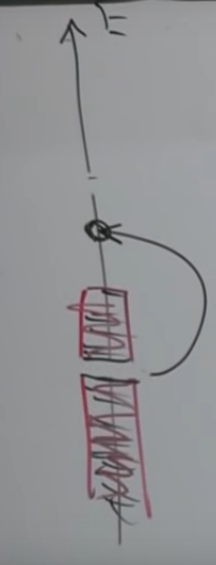
\includegraphics[width=0.4\textwidth]{DiracSea}
	\end{center}
\end{figure}

Imagine photon coming along and hitting -ve energy electron in vacuum: we get an electron and a hole--Figure \ref{photon:dirac}.

\begin{figure}
	\begin{center}
		\caption[Photon$\rightarrow$ electrons + hole]{Photon$\rightarrow$ electons + hole. By convention positron points down. Can slice in time: upwards electron, down positrons.}\label{photon:dirac}
		\feynmandiagram[vertical=o2 to i1]{
			i1--[photon,edge label=$\gamma$]n1--[anti fermion]o1[particle=$e^+$],
			n1--[fermion]o2[particle=$e^-$]
		};
	\end{center}
\end{figure}

The wave function needs fermion operators, which anticommute.
\begin{align*}
\Psi =& \int_{-\infty}^{\infty} dp a^-(p) e^{-ipx}\\
=& \underbrace{\int_{-\infty}^0 dp a^-(p) e^{-ipx}}_\text{negative energies}+ \underbrace{\int_0^{\infty} dp a^-(p) e^{-ipx}}_\text{positive energies}\\
=&  \underbrace{\int_0^{\infty} dp b^+(p) e^{ipx}}_\text{Creation operator for positron}+ \int_0^{\infty} dp a^-(p) e^{-ipx}
\end{align*}

Since Fermion creation and annihilation operators the same.

Consider the interaction of Figure \ref{fig:electron_scattering_dirac}.
\begin{align*}
a^+a^-A& \text{, which comes from a term in the Hamiltonian:}\\
\Psi^\dagger(x)\Psi(x)A&\text{, }
\end{align*}

But this also describes the interactions of  Figures \ref{fig:electron_scattering_dirac}, \ref{fig:positron annihilating_dirac}, and \ref{fig:all3-created}.
\begin{figure}[H]
	\caption{Possible outcomes of $\Psi^\dagger(x)\Psi(x)A$: Feynman diagrams}
	\begin{subfigure}{0.3\textwidth}
		\caption{Electron scattering}\label{fig:electron_scattering_dirac}
		\feynmandiagram[vertical=o2 to i1]{
			i1[particle=$e^-$]--[fermion]a--[fermion]o1[particle=$e^-$],
			a--[photon]o2
		};
	\end{subfigure}
	\begin{subfigure}{0.3\textwidth}
		\caption{Positron annihilation}\label{fig:positron annihilating_dirac}
		\feynmandiagram[vertical=a to i1]{
			i1[particle=$e^-$]--[fermion]a--[boson]o1,
			i2[particle=$e^+$]--[anti fermion]a
		};
	\end{subfigure}
	\begin{subfigure}{0.3\textwidth}
		\caption{Electron, photon, positron created}\label{fig:all3-created}
		\feynmandiagram[vertical=o2 to i1]{
			i1--[fermion]o1[particle=$e^-$],
			i1--[boson]o2,
			i1--[anti fermion]o3[particle=$e^+$]
		};
	\end{subfigure}
\end{figure}

Same pattern in solid state physics. If you have crystal with lots of electrons, put all electrons into lowest available states--ground state. We have the Fermi sea. Can take an energy out of sea and kick into higher state, leaving a hole which behaves like a particle. But Dirac did this first!

\bibliographystyle{unsrt}
\addcontentsline{toc}{section}{Bibliography}
\raggedright
\bibliography{tm}

\end{document}